% Ensemble Composition Ablation: MAE by Configuration
% Replaces: tab:ensemble-composition-results in appendix_c
% Shows diminishing returns as models are added

\begin{figure}[htbp]
\centering
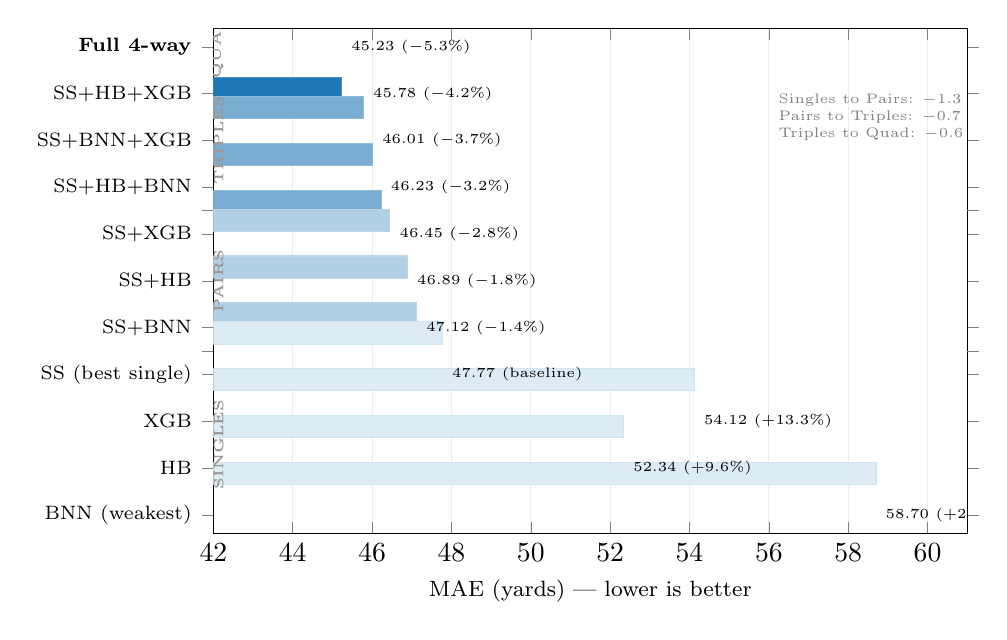
\begin{tikzpicture}
\definecolor{accent}{RGB}{31,119,180}

\begin{axis}[
  width=0.92\textwidth,
  height=8cm,
  xbar,
  bar width=8pt,
  xmin=42, xmax=61,
  xlabel={MAE (yards) --- lower is better},
  xlabel style={font=\footnotesize},
  ytick={1,2,3,4,5,6,7,8,9,10,11},
  yticklabels={
    {\textbf{Full 4-way}},
    SS+HB+XGB,
    SS+BNN+XGB,
    SS+HB+BNN,
    SS+XGB,
    SS+HB,
    SS+BNN,
    {SS (best single)},
    XGB,
    HB,
    {BNN (weakest)}
  },
  yticklabel style={font=\scriptsize},
  y dir=reverse,
  grid=major,
  grid style={gray!15},
  xmajorgrids=true,
  ymajorgrids=false,
  enlarge y limits={abs=0.4},
  % Group separators
  extra y ticks={4.5, 7.5},
  extra y tick labels={},
  extra y tick style={grid style={black!30, dashed}},
]

% Full ensemble (highlighted)
\addplot[fill=accent, draw=accent!80] coordinates {(45.23, 1)};

% Triples
\addplot[fill=accent!60, draw=accent!50] coordinates {
  (45.78, 2) (46.01, 3) (46.23, 4)
};

% Pairs
\addplot[fill=accent!35, draw=accent!30] coordinates {
  (46.45, 5) (46.89, 6) (47.12, 7)
};

% Singles
\addplot[fill=accent!15, draw=accent!20] coordinates {
  (47.77, 8) (54.12, 9) (52.34, 10) (58.70, 11)
};

% Value labels
\node[font=\tiny, anchor=west] at (axis cs:45.23,1) {45.23 ($-$5.3\%)};
\node[font=\tiny, anchor=west] at (axis cs:45.78,2) {45.78 ($-$4.2\%)};
\node[font=\tiny, anchor=west] at (axis cs:46.01,3) {46.01 ($-$3.7\%)};
\node[font=\tiny, anchor=west] at (axis cs:46.23,4) {46.23 ($-$3.2\%)};
\node[font=\tiny, anchor=west] at (axis cs:46.45,5) {46.45 ($-$2.8\%)};
\node[font=\tiny, anchor=west] at (axis cs:46.89,6) {46.89 ($-$1.8\%)};
\node[font=\tiny, anchor=west] at (axis cs:47.12,7) {47.12 ($-$1.4\%)};
\node[font=\tiny, anchor=west] at (axis cs:47.77,8) {47.77 (baseline)};
\node[font=\tiny, anchor=west] at (axis cs:54.12,9) {54.12 (+13.3\%)};
\node[font=\tiny, anchor=west] at (axis cs:52.34,10) {52.34 (+9.6\%)};
\node[font=\tiny, anchor=west] at (axis cs:58.70,11) {58.70 (+22.9\%)};

% Group labels
\node[font=\tiny\bfseries, text=black!40, rotate=90, anchor=south] at (axis cs:42.5,1) {QUAD};
\node[font=\tiny\bfseries, text=black!40, rotate=90, anchor=south] at (axis cs:42.5,3) {TRIPLES};
\node[font=\tiny\bfseries, text=black!40, rotate=90, anchor=south] at (axis cs:42.5,6) {PAIRS};
\node[font=\tiny\bfseries, text=black!40, rotate=90, anchor=south] at (axis cs:42.5,9.5) {SINGLES};

% Diminishing returns annotation
\node[font=\tiny, text=black!50, anchor=west, align=left] at (axis cs:56,2.5)
  {Singles to Pairs: $-$1.3 yd\\Pairs to Triples: $-$0.7 yd\\Triples to Quad: $-$0.6 yd};

\end{axis}
\end{tikzpicture}
\caption[Ensemble composition ablation]{Ensemble composition ablation (2022--2024, $n=1{,}405$ QB-games). Adding models consistently improves MAE but with diminishing returns: the full 4-way ensemble achieves 45.23 yards MAE, 5.3\% better than the best single model. Even the weakest component (BNN) contributes 1.2\% improvement when added to the 3-way ensemble. Percentages are relative to the State-Space v2 baseline.}
\label{fig:ablation-composition-chart}
\end{figure}
